% Generated standalone skeleton. Layout authority: templates/mcm-style.tex via scripts.paper_template.
% Reuse this layout for MCM reports; metadata/content may change, style overrides must be reviewed.
% Run: uv run --locked python -m scripts.paper_template main.tex
% Canonical build: uv run --locked python -m scripts.paper_template main.tex --contest mcm --compile --output-directory outputs/build-001
% Layout profile is a project convention, not the official rules for any year.
% Before formal submission verify the selected edition's Summary Sheet, page limit,
% anonymity and AI disclosure requirements; do not inherit a historical edition.
% Check layout: uv run --locked python -m scripts.paper_template main.tex
\newcommand{\PraxisTeam}{0000000}
\newcommand{\PraxisTitle}{Title: state the answer, not the topic}
% BEGIN PRAXIS MCM STYLE v1
% Praxis MCM house style v1. Layout source; assemble with scripts.paper_template.
\documentclass[12pt,letterpaper]{article}
\usepackage[left=1in,right=1in,top=0.95in,bottom=0.8in,headheight=15pt]{geometry}
\usepackage{amsmath,amssymb,amsthm}
\usepackage{newtxtext,newtxmath}
\usepackage{booktabs,array,graphicx,xcolor,caption,float,etoolbox,fvextra,fancyhdr,lastpage,titlesec,titletoc,needspace}
\usepackage[hidelinks,pdfauthor={},pdftitle={\PraxisTitle}]{hyperref}
\urlstyle{same}\Urlmuskip=0mu plus 1mu
\usepackage{pgfplots}
\pgfplotsset{compat=1.17}
\usepgfplotslibrary{fillbetween,groupplots}
\usetikzlibrary{arrows.meta,positioning,calc}
\definecolor{main}{HTML}{0072B2}
\definecolor{accent}{HTML}{D55E00}
\definecolor{muted}{HTML}{7A7F85}
\definecolor{light}{HTML}{B8BDC2}
\definecolor{oigreen}{HTML}{009E73}
\definecolor{oiorange}{HTML}{E69F00}
\definecolor{oisky}{HTML}{56B4E9}
\definecolor{oiyellow}{HTML}{F0E442}
\definecolor{teal}{HTML}{17766E}
\definecolor{clay}{HTML}{9E6440}
\definecolor{slate}{HTML}{5D696E}
\definecolor{sand}{HTML}{AAA69B}
\linespread{1.12}
\setlength{\parindent}{1.5em}\setlength{\parskip}{3pt}
\titleformat{\section}{\Large\bfseries}{\thesection}{0.6em}{}
\titleformat{\subsection}{\large\bfseries}{\thesubsection}{0.6em}{}
\titlespacing*{\section}{0pt}{16pt plus 3pt}{8pt}
\titlespacing*{\subsection}{0pt}{12pt plus 2pt}{6pt}
\captionsetup{font=small,labelfont=bf,labelsep=period,justification=centering}
\captionsetup[table]{position=above,skip=5pt}\captionsetup[figure]{position=below,skip=7pt}
\setcounter{tocdepth}{2}
\setlength{\emergencystretch}{3em}
\pagestyle{fancy}\fancyhf{}
\fancyhead[L]{Team \# \PraxisTeam}\fancyhead[R]{Page \thepage{} of \pageref{LastPage}}
\renewcommand{\headrulewidth}{0.4pt}
\makeatletter\setlength{\@fptop}{0pt}\setlength{\@fpsep}{14pt}\setlength{\@fpbot}{0pt plus 1fil}\makeatother
\AtBeginEnvironment{thebibliography}{\small}
% Two visible levels; both use aligned dot leaders, with hierarchy by weight/indent.
\titlecontents{section}[1.8em]{\addvspace{5pt}\bfseries}{\contentslabel{1.8em}}{}{\titlerule*[.6pc]{.}\contentspage}
\titlecontents{subsection}[4.1em]{}{\contentslabel{2.3em}}{}{\titlerule*[.6pc]{.}\contentspage}
% END PRAXIS MCM STYLE
\begin{document}
\thispagestyle{empty}\begin{center}\begin{tabular*}{\linewidth}{@{\extracolsep{\fill}}ccc}
\textbf{Problem Chosen}&\textbf{MCM/ICM}&\textbf{Team Control Number}\\
{\Large\textbf{A}}&\shortstack{\textbf{Summary Sheet}\\Page \thepage{} of \pageref{LastPage}}&{\Large\textbf{\PraxisTeam}}\end{tabular*}\end{center}\vspace{-4pt}\hrule\vspace{10pt}
\begin{center}{\LARGE\bfseries Title: state the answer, not the topic}\end{center}
\begin{center}{\Large\bfseries Summary}\end{center}
Write this page last: the problem, the main model, quantitative results with units, validation, limits and the recommendation.\par
\textbf{Keywords:} keyword one; keyword two

\clearpage\tableofcontents\clearpage
\section{Define the decision before optimizing}
Each requirement of the problem statement maps to a result, a figure and a section.

\section{Assumptions, data and parameters}
Every assumption has a reason; every parameter has a source and a range.
\begin{table}[htbp]\centering\small\caption{Parameters, sources and ranges}
\begin{tabular}{llll}\toprule Symbol & Meaning & Value (range) & Source\\ \midrule $k$ & example & 1.0 (0.5--2) & [1]\\ \bottomrule\end{tabular}\end{table}

\section{Model and results}
\begin{equation}J=\int_0^{t_f} q(t)\,dt\end{equation}
% A figure drawn from data: python -c "from scripts import texplot; ..." writes the axis source.
\begin{figure}[htbp]\centering
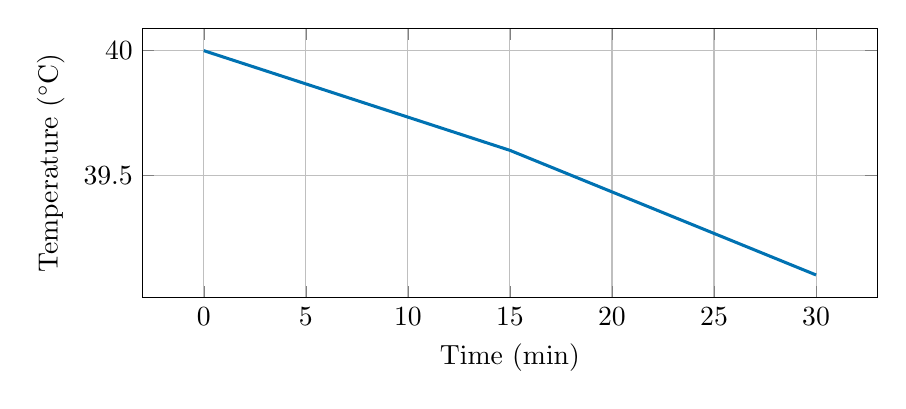
\begin{tikzpicture}
\begin{axis}[width=0.9\linewidth,height=5cm,xlabel={Time (min)},ylabel={Temperature ($^\circ$C)},grid=major]
\addplot[color=main,line width=1.1pt,no marks] coordinates {(0,40) (15,39.6) (30,39.1)};
\end{axis}
\end{tikzpicture}
\caption{One sentence on what the reader should see.}\end{figure}

\section{Validation, sensitivity and limits}
Compare with a simple baseline, perturb parameters and execution, and state what the model cannot support.

\section{Conclusions and recommendation}

\clearpage\section*{References}\addcontentsline{toc}{section}{References}
\begingroup\small\setlength{\parindent}{0pt}\hangindent=1.5em
[1] Author. Title. Publisher, year. \url{https://example.org/}\par
\endgroup
\clearpage\section*{Report on Use of AI}\addcontentsline{toc}{section}{Report on Use of AI}
Name each tool and version, what it did, what was adopted or changed, how outputs were verified, and what the record cannot show.
\end{document}
